\documentclass{report}

\usepackage{amsfonts, amsmath, amssymb}
\usepackage{mathtools}

\newcommand{\E}{\mathrm{E}}
\newcommand{\Var}{\mathrm{Var}}
\newcommand{\Cov}{\mathrm{Cov}}
\newcommand{\e}{\text{e}}

\title{FinPy \\[0.4cm] \Large Financial engineering library for Python}

\begin{document}

\maketitle

\tableofcontents

% \chapter{Introduction}

% \chapter{Models}

\chapter{1-Factor Hull-White}

\section{Definitions}

The price of a zero-coupon bond maturing at time $t$, $P(0,t)$, is related to the continuously compounded yield
\begin{equation}
P(0,t) = \e^{-y(0,0,t) t}.
\end{equation}

\begin{equation}
P(0,t) = \exp \left( -\int_0^t f(0,u) du \right).
\end{equation}
Thus
\begin{equation}
f(t,T) = - \frac{\partial \ln P(t,T)}{\partial T}.
\end{equation}


\section{Tests of implementation...}

The Monte-Carlo simulation is based on the pseudo short rate $x(t)$ defined by
\begin{equation}
x(t) = r(t) - f(0,t),
\end{equation}
where $x(0) = 0$.

The corresponding pseudo discount function is given by
\begin{equation}
X(t) = \exp \left( - \int_0^t x(u) du \right)
\end{equation}
hence, the real discount function is given by
\begin{equation}
D(t) = \exp \left( - \int_0^t r(u) du \right) = P(0,t) \exp \left( - \int_0^t x(u) du \right) = P(0,t) X(t).
\end{equation}


\begin{figure}
\centering
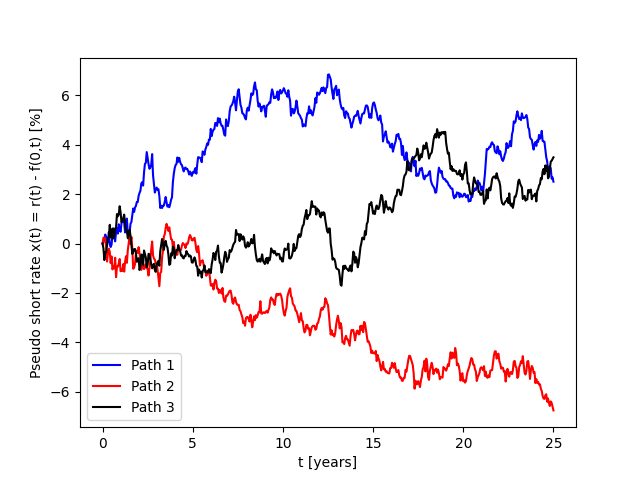
\includegraphics[scale=0.7]{figures/pseudo_short_rate_paths.png}
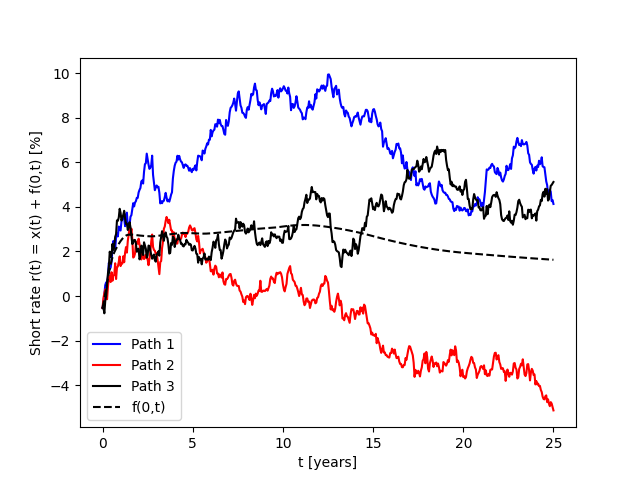
\includegraphics[scale=0.7]{figures/short_rate_paths.png}
\caption{Monte-Carlo paths for $x(t)$ and $r(t)$...}
\end{figure}

\begin{figure}
\centering
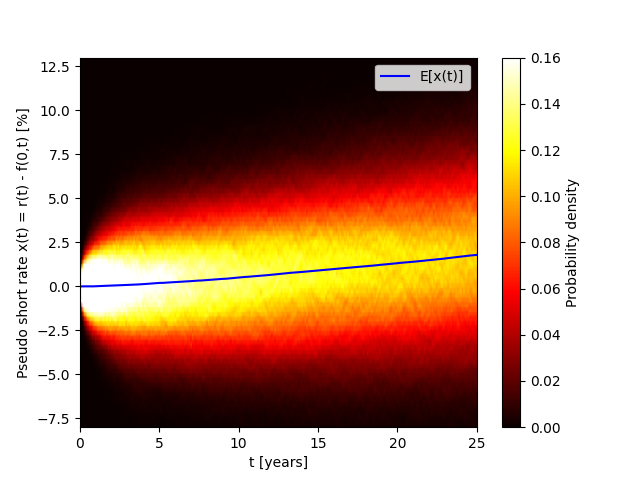
\includegraphics[scale=0.7]{figures/pseudo_short_rate_density.png}
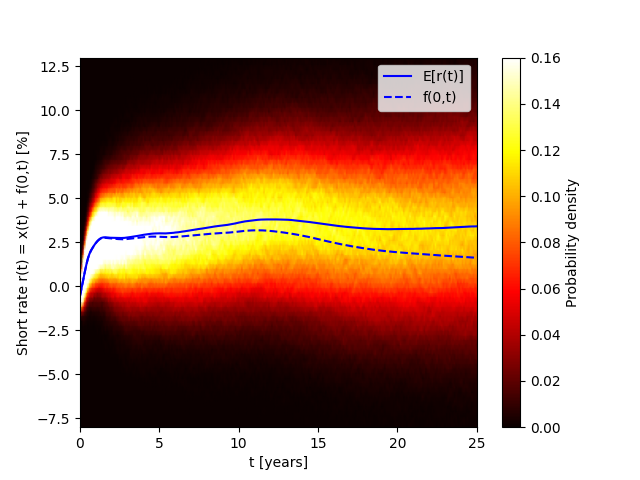
\includegraphics[scale=0.7]{figures/short_rate_density.png}
\caption{Density plots of $x(t)$ and $r(t)$...}
\end{figure}

\begin{figure}
\centering
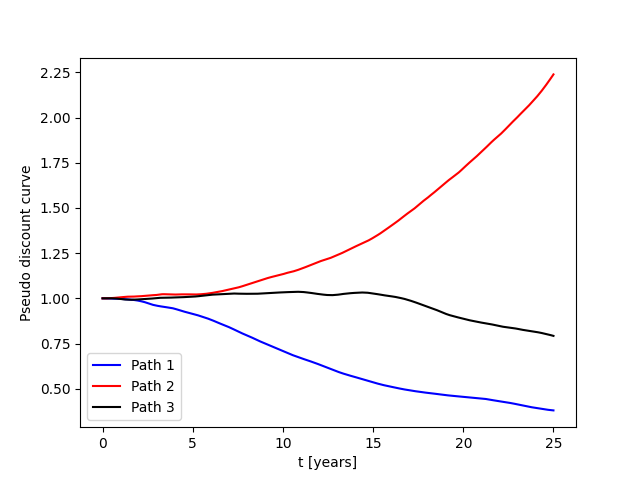
\includegraphics[scale=0.7]{figures/pseudo_discount_paths.png}
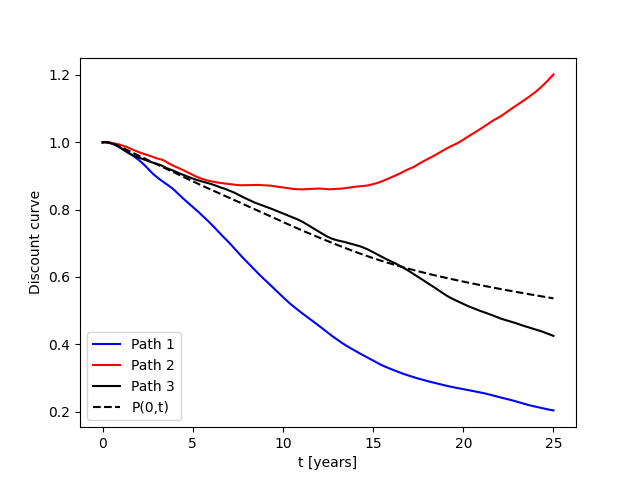
\includegraphics[scale=0.7]{figures/discount_paths.png}
\caption{Monte-Carlo paths for $X(t)$ and $D(t)$...}
\end{figure}

\begin{figure}
\centering
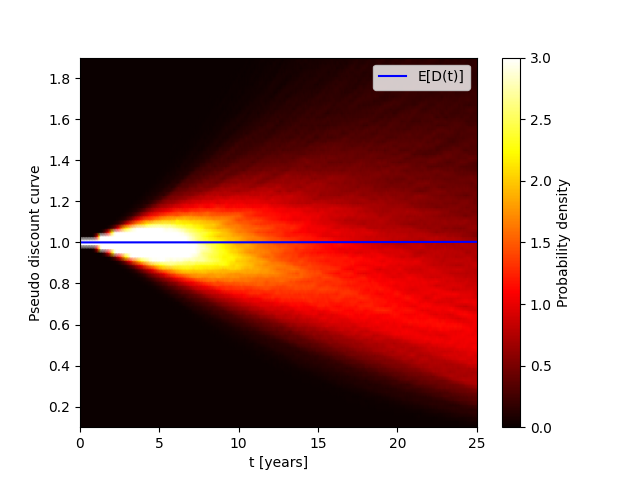
\includegraphics[scale=0.7]{figures/pseudo_discount_density.png}
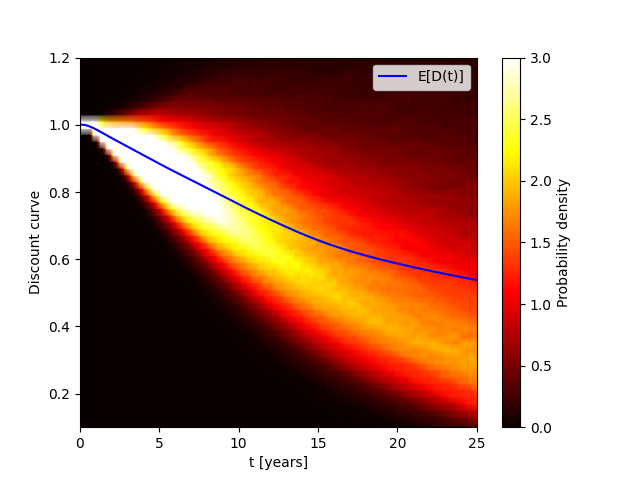
\includegraphics[scale=0.7]{figures/discount_density.png}
\caption{Density plots of $X(t)$ and $D(t)$...}
\end{figure}

\section{Tests of Monte-Carlo convergence}

\appendix

\chapter{Short Rate Models}

\section{Vasicek Model}
The Vasicek model \cite{Vasicek1977} is a short rate model defined by the stochastic differential equation 
\begin{equation}
dr_t = \kappa \left( \theta - r_t \right) dt + \sigma dW_t,
\end{equation}
where $\kappa > 0$ is the speed of mean reversion, $\theta$ denotes the long-term level, and $\sigma > 0$ is the volatility.
As usual, $W_t$ denotes the Wiener process under the risk-neutral $Q$-measure.

The SDE can be solved analytically by introducing the function
\begin{equation}
h(t, r_t) = r_t \e^{\kappa t},
\end{equation}
using It\^{o}'s lemma
\begin{eqnarray}
dh(t, r_t) &=& \frac{\partial h}{\partial t} dt + \frac{\partial h}{\partial r_t} dr_t + \frac{1}{2}\frac{\partial^2 h}{\partial r_t^2} \left(dr_t\right)^2 \\
&=& \kappa h(t, r_t) dt + \e^{\kappa t} dr_t \\
&=& \theta \kappa \e^{\kappa t} dt + \sigma \e^{\kappa t} dW_t,
\end{eqnarray}
and integrating from $t_1$ to $t_2$
\begin{equation}
h(t_2, r_{t_2}) = h(t_1, r_{t_1}) + \theta \kappa \int_{t_1}^{t_2} \e^{\kappa t} dt + \sigma \int_{t_1}^{t_2} \e^{\kappa t} dW_t,
\end{equation}
such that ($\Delta t \coloneq t_2 - t_1$)
\begin{equation}
r_{t_2} = \theta + \left( r_{t_1} - \theta \right) \e^{-\kappa \Delta t} + \sigma \int_{t_1}^{t_2} \e^{-\kappa \left(t_2 - t\right)} dW_t.
\end{equation}

The short rate process is clearly Gaussian with conditional mean (the expectation operator is defined with respect to the $Q$-measure)
\begin{equation}
\E \left[ r_{t_2} | r_{t_1} \right] = \theta + \left( r_{t_1} - \theta \right) \e^{-\kappa \Delta t},
\end{equation}
and, using the It\^{o} isometry, the conditional variance of the process becomes
\begin{eqnarray}
\Var \left[ r_{t_2} | r_{t_1} \right] &=& \E \left[ \left( \sigma \int_{t_1}^{t_2} \e^{-\kappa \left(t_2 - t\right)} dW_t \right)^2 \right] \\
&=& \frac{\sigma^2}{2 \kappa} \left( 1 - \e^{-2 \kappa \Delta t}\right).
\end{eqnarray}

The stochastic discount factor is written as
\begin{equation}
D_{t} = \exp \left( I_t \right),
\end{equation}
where
\begin{eqnarray}
I_t &=& -\int_0^t r_u du \\
&=& - \int_0^t \left( \theta + \left( r_0 - \theta \right) \e^{-\kappa u } \right) du - \sigma \int_0^t \int_0^u \e^{-\kappa \left(u - v\right)} dW_v du \\
&=& - \theta t - \frac{r_0 - \theta}{\kappa} \left( 1 - \e^{-\kappa t} \right) - \sigma \int_0^t \int_v^t \e^{-\kappa \left(u - v\right)} du dW_v.
\end{eqnarray}

The conditional mean of $I_t$ is
\begin{equation}
\E \left[ I_{t_{2}} | I_{t_1}, r_{t_1} \right] = I_{t_1} - \theta \Delta t 
- \frac{r_{t_1} - \theta}{\kappa} \left( 1 - \e^{-\kappa \Delta t} \right),
\end{equation}
and, using the It\^{o} isometry, the conditional variance becomes
\begin{eqnarray}
\Var \left[ I_{t_{2}} | I_{t_1}, r_{t_1} \right] &=& \E \left[ \left( \sigma \int_{t_1}^{t_2} \int_v^{t_2} \e^{-\kappa \left(u - v\right)} du dW_v \right)^2 \right] \\
&=& \frac{\sigma^2}{2 \kappa^3} \left( 4 \e^{-\kappa \Delta t} - \e^{-2\kappa \Delta t} + 2 \kappa \Delta t - 3 \right)
\end{eqnarray}

We can write both $r_t$ and $I_t$ as a sum of a deterministic term ($D$) and a stochastic term ($S$)
\begin{eqnarray}
r_t &=& D_{r_t} + S_{r_t} \\
I_t &=& D_{I_t} + S_{I_t},
\end{eqnarray}
such that the covariance of $r_t$ and $I_t$ is expressed as
\begin{eqnarray}
\Cov \left[ r_t, I_t \right] &=& \E \left[ r_t I_t \right] - \E \left[ r_t \right] \E \left[ I_t \right] \\
&=& \E \left[ D_{r_t} D_{I_t} + S_{r_t} D_{I_t} + D_{r_t} S_{I_t} + S_{r_t} S_{I_t} \right] - D_{r_t} D_{I_t} \\
&=& \E \left[ S_{r_t} S_{I_t} \right].
\end{eqnarray}

\begin{eqnarray}
\Cov \left[ r_t, I_t \right] &=& - \sigma^2 \E \left[ \int_0^t \e^{-\kappa (t - u)} dW_u \int_0^t \int_v^t \e^{-\kappa(u-v)} du dW_v \right] \\
&=& -\sigma^2 \int_0^t \E \left[ \e^{-\kappa(t-v)} \int_v^t \e^{-\kappa(u-v)} du \right] dv \\
&=& \frac{\sigma^2}{2 \kappa^2} \left( 2 \e^{-\kappa t} - \e^{-2\kappa t} - 1 \right).
\end{eqnarray}

The price of a $T$-maturity zero-coupon bond at time $t$ is given by
\begin{eqnarray}
P(t,T) &=& \E \left[ \exp \left(\text{e}^{I_T - I_t} \right) \right] \\
&=& \exp \left( \E \left[ \text{e}^{I_T - I_t} \right] + \frac{1}{2} \Var \left[ \text{e}^{I_T - I_t} \right] \right) \\
&=& \exp \left( A(t,T) - B(t,T) r_t \right) ,
\end{eqnarray}
where
\begin{eqnarray}
A(t,T) &=& \left( \theta - \frac{\sigma^2}{2 \kappa^2} \right) \left( B(t,T) - (T- t)\right) - \frac{\sigma^2}{4 \kappa} B(t,T)^2 \\
B(t,T) &=& \frac{1 - \text{e}^{-\kappa (T-t)}}{\kappa}.
\end{eqnarray}

Closed form pricing functions for European call and put options written on zero-coupon bonds can also be derived, see REF X.

\subsection{Transformation to short rate representation}

Zero-coupon bond prices and instantaneous forward rates are related by
\begin{equation}
P(0,t) = \e^{- \int_0^t f(0,u) du}.
\end{equation}

Using the transformation of the short rate in Eq.~X, we get that
\begin{eqnarray}
P(0,t) &=& \E \left[ \e^{- \int_0^t r_u du} \right] \\
&=& \e^{- \int_0^t f(0,u) du} \E \left[ \e^{- \int_0^t x_u du} \right],
\end{eqnarray}
which implies that
\begin{equation}
\E \left[ \e^{- \int_0^t x_u du} \right] = 1.
\end{equation}

Also for a given scenario, i.e., $r_t(\omega) = x_t (\omega) + f(0,t)$, we get
\begin{equation}
\e^{- \int_0^t r_u (\omega) du} = P(0,t) \e^{- \int_0^t x_u (\omega) du}.
\end{equation}


\section{1-Factor Hull-White Model}
The 1-Factor Hull-White model REF! is an extension of the Vasicek Model, where the parameters are allowed to be time-dependent, i.e.,
\begin{equation}
dr_t = \kappa_t \left( \theta_t - r_t \right) dt + \sigma_t dW_t.
\end{equation}

The $\theta_t$ is chosen such that the short rate model is consistent with the initial yield curve.

We define $x_t = r_t - f(0,t)$ such that
\begin{equation}
dx_t = \left( y_t - \kappa_t r_t \right) dt + \sigma_t dW_t,
\label{eq:HullWhiteSDEx}
\end{equation}
where
\begin{equation}
y_y = \int_0^t \e^{-2\int_u^t \kappa_s ds} \sigma_u^2 du.
\end{equation}

The SDE in Eq.~(\ref{eq:HullWhiteSDEx}) can be solved analytically by introducing the function
\begin{equation}
h(t, x_t) = x_t \e^{\int_0^t \kappa_u du}
\end{equation}
using It\^{o}'s lemma
\begin{eqnarray}
dh(t, x_t) &=& \frac{\partial h}{\partial t} dt + \frac{\partial h}{\partial x_t} dx_t + \frac{1}{2}\frac{\partial^2 h}{\partial x_t^2} \left(dx_t\right)^2 \\
&=& \kappa_t h(t, x_t) dt + \e^{\kappa t} dx_t \\
&=& y_t \e^{\int_0^t \kappa_u du} dt + \sigma_t \e^{\int_0^t \kappa_u du} dW_t,
\end{eqnarray}
and integrating from $t_1$ to $t_2$
\begin{equation}
h(t_2, r_{t_2}) = h(t_1, r_{t_1}) + \int_{t_1}^{t_2} y_t \e^{\int_0^t \kappa_u du} dt + \int_{t_1}^{t_2} \sigma_t \e^{\int_0^t \kappa_u du} dW_t,
\end{equation}
such that
\begin{equation}
x_{t_2} = x_{t_1} \e^{-\int_{t_1}^{t_2} \kappa_u du}  + \int_{t_1}^{t_2} y_t \e^{-\int_t^{t_2} \kappa_u du} dt + \int_{t_1}^{t_2} \sigma_t \e^{-\int_t^{t_2} \kappa_u du} dW_t.
\end{equation}

The pseudo short rate process is clearly Gaussian with conditional mean (the expectation operator is defined with respect to the $Q$-measure)
\begin{equation}
\E \left[ x_{t_2} | x_{t_1} \right] = x_{t_1} \e^{-\int_{t_1}^{t_2} \kappa_u du}  + \int_{t_1}^{t_2} y_t \e^{-\int_t^{t_2} \kappa_u du} dt,
\end{equation}
and, using the It\^{o} isometry, the conditional variance of the process becomes
\begin{eqnarray}
\Var \left[ x_{t_2} | x_{t_1} \right] &=& \E \left[ \left( \int_{t_1}^{t_2} \sigma_t \e^{-\int_t^{t_2} \kappa_u du} dW_t \right)^2 \right] \\
&=& \int_{t_1}^{t_2} \sigma_t^2 \e^{-2\int_t^{t_2} \kappa_u du} dt.
\end{eqnarray}

The stochastic pseudo discount factor is written as
\begin{equation}
D_{t} = \exp \left( I_t \right),
\end{equation}
where
\begin{eqnarray}
I_t &=& -\int_0^t x_u du \\
&=& - x_{0} \int_0^t \e^{-\int_{0}^{u} \kappa_v dv} du - \int_0^t\int_{0}^{u} y_v \e^{-\int_v^{u} \kappa_s ds} dv du \\
&& - \int_0^t \int_{0}^{u} \sigma_v \e^{-\int_v^{u} \kappa_s ds} dW_v du.
\end{eqnarray}

The conditional mean of $I_t$ is
\begin{equation}
\E \left[ I_{t_{2}} | I_{t_1}, r_{t_1} \right] = I_{t_1} - x_{t_1} \int_{t_1}^{t_2} \e^{-\int_{0}^{u} \kappa_v dv} du - \int_{t_1}^{t_2} \int_{0}^{u} y_v \e^{-\int_v^{u} \kappa_s ds} dv du,
\end{equation}
and, using the It\^{o} isometry, the conditional variance becomes
\begin{eqnarray}
\Var \left[ I_{t_{2}} | I_{t_1}, r_{t_1} \right] &=& \E \left[ \left( \int_0^t \int_{0}^{u} \sigma_v \e^{-\int_v^{u} \kappa_s ds} dW_v du \right)^2 \right].
\end{eqnarray}

% Bibliography
\bibliographystyle{plain}
\bibliography{articles} 

\end{document}